%%%%%%%%%%%%%%%%%%%%%%%%%%%%%%%%%%%%%%%%%%%%%%%%%%%%%%%%%%%%%%%%%%% 
%                                                                 %
%                           CHAPTER 4                             %
%                                                                 %
%%%%%%%%%%%%%%%%%%%%%%%%%%%%%%%%%%%%%%%%%%%%%%%%%%%%%%%%%%%%%%%%%%% 
 
\chapter{The tropopause-layer static stability structure of tropical cyclones: Idealized modeling}
\resetfootnote %this command starts footnote numbering with 1 again.

%---------------------------------------------------------------------------------------%
\section{Introduction}
%---------------------------------------------------------------------------------------%

The preceding two chapters highlighted the effect of tropical cyclones on the tropopause and upper-level static stability structure in dropsonde observations.
These observations alone, however, cannot explain the mechanisms that force the observed variability.
Numerical simulations of an axisymmetric hurricane conducted in an idealized framework reproduced the observed variability.
Using these simulations, some physical insight into these mechanisms is obtained and described in the present chapter.

%---------------------------------------------------------------------------------------%
\section{Model Setup}
%---------------------------------------------------------------------------------------%

The numerical simulations were performed using version 19.4 of Cloud Model 1 (CM1) described in \cite{BryanRotunno2009}.
The equations of motion were integrated on a 3000-km-wide, 30-km-deep axisymmetric grid with 1-km horizontal and 250-m vertical grid spacing.
The computations were performed on an \textit{f}-plane at 15\textdegree{N} latitude, over a sea surface with constant temperature of 30.5\textdegree C, which matches that observed near Hurricane Patricia (2015; \citeauthor{Kimberlainetal2016} \citeyear{Kimberlainetal2016}).
Horizontal turbulence was parameterized using the Smagorinsky scheme described in \citeauthor{BryanRotunno2009} (\citeyear{BryanRotunno2009}, pg. 1773), with a prescribed mixing length that varied linearly from 100 m at a surface pressure of 1015 hPa to 1000 m at a surface pressure of 900 hPa.
Vertical turbulence was parameterized using the formulation of \citeauthor{MarkowskiBryan2016} (\citeyear{MarkowskiBryan2016}, their Eq. 6), using an asymptotic vertical mixing length of 100 m.
A Rayleigh damping layer was applied outside of the 2900-km radius and above the 25-km level to prevent spurious gravity wave reflection at the model boundaries.
Microphysical processes were parameterized using the \cite{Thompson} scheme and radiative heating tendencies were computed every two minutes using the Rapid Radiative Transfer Model for GCMs (RRTMG) longwave and shortwave schemes \citep{Iacono}.
The initial temperature and humidity field was horizontally homogeneous and determined by averaging all Climate Forecast System Reanalysis (CFSR) grid points within 100 km of Patricia's center of circulation at 18 UTC 21 October 2015.
%A horizontally-homogeneous temperature and humidity field was initialized with a mean sounding computed using all dropsondes deployed during the TCI flight conducted within and around Tropical Storm Patricia on 21 October, 2015 (see \citeauthor{DoyleTCI} \citeyear{DoyleTCI} for details.)
%Above 19 km, where few TCI observations were available, the temperature profile was taken from the Climate Forecast System Reanalysis (CFSR) grid point nearest Patricia's storm center, valid at 18 UTC 21 October, 2015.
%Since relative humidity measurements were unreliable at temperatures below -40\textdegree C \citep{BellTCI}, relative humidity was set equal to 50\% above 11.5 km (the level above which temperature dropped below -40\textdegree C).
The vortex described in \citeauthor{RotunnoEmanuel} (\citeyear{RotunnoEmanuel}, their Eq. 37) was used to initialize the wind field, setting all parameters equal to the values used therein.

Although hurricanes simulated in an axisymmetric framework tend to be more intense than those observed in nature, the intensity evolution of this simulation matches reasonably well with that observed in Hurricane Patricia.
After an initial spin-up period of about 20 hours, the modeled storm (Fig.~\ref{fig:vmax+pmin}, blue lines) began an RI period that lasted approximately 30 hours.
After this RI, the storm continued to intensify more slowly until the maximum 10-m wind speed reached 89 m s\textsuperscript{-1} and the sea-level pressure reached its minimum of 846 hPa 81 hours into the simulation.
Hurricane Patricia (red stars) exhibited a similar intensity evolution prior to its landfall, with an RI period leading to a maximum 10-m wind speed of 95 m s\textsuperscript{-1} and a minimum sea-level pressure of 872 hPa.

%---------------------------------------------------------------------------------------%
\section{Budget Computation}
%---------------------------------------------------------------------------------------%
The static stability can be expressed as the squared Brunt-V{\"a}is{\"a}l{\"a} frequency:
   \begin{equation} \label{eq:n2moist}
   N_m^2 = \frac{g}{T}\left(\frac{\partial T}{\partial z}+\Gamma_m\right)\left(1+\frac{T}{R_d/R_v+q_s}\frac{\partial q_s}{\partial T}\right)-\frac{g}{1+q_t}\frac{\partial q_t}{\partial z},
   \end{equation}
where $g$ is gravitational acceleration, $T$ is temperature, $R_d$ and $R_v$ are the gas constants of dry air and water vapor, respectively, $q_s$ is the saturation mixing ratio, $q_t$ is the total condensate mixing ratio, and $\Gamma_m$ is the moist-adiabatic lapse rate:
   \begin{equation} \label{eq:gamma_m}
   \Gamma_m = g(1+q_t)\left(\frac{1+L_vq_s/R_dT}{c_{pm}+L_v\partial q_s/\partial T}\right),
   \end {equation}
where $L_v$ is the latent heat of vaporization and $c_{pm}$ is the specific heat of moist air at constant pressure.
In the tropopause layer, $q_s$, ${\partial q_s}/{\partial T}$, and ${\partial q_t}/{\partial z}$ approach zero. In this limiting case, Eq. \ref{eq:n2moist} reduces to:
   \begin{equation} \label{eq:n2dry}
   N^2 = \frac{g}{\theta}\frac{\partial \theta}{\partial z},
   \end{equation}
where $\theta$ is the potential temperature.

To compute $N^2$, CM1 uses Eq. \ref{eq:n2moist} in saturated environments and Eq. \ref{eq:n2dry} in sub-saturated environments. For simplicity, however, only Eq. \ref{eq:n2dry} will be employed for the budget computations throughout the entire domain\footnote{The validity of this approximation will be substantiated later in this section.}.

Taking the time derivative of Eq. \ref{eq:n2dry} yields the static stability tendency:
   \begin{equation} \label{eq:dn2dt}
   \frac{\partial N^2}{\partial t} = \frac{g}{\theta}\frac{\partial}{\partial z}\frac{\partial \theta}{\partial t}-\frac{g}{\theta^2}\frac{\partial \theta}{\partial z}\frac{\partial \theta}{\partial t},
   \end{equation}
where the potential temperature tendency, $\partial \theta/\partial t$, can be written, following \cite{Bryan2017}:
   \begin{equation} \label{eq:dthetadt}
%   \frac{\partial \theta}{\partial t} = HADV+VADV+HTURB+VTURB+MP+RAD+DISS 
   \frac{\partial \theta}{\partial t} = -u\frac{\partial\theta}{\partial r}-w\frac{\partial \theta}{\partial z}+HTURB+VTURB+MP+RAD+DISS
   \end{equation}
Each term on the right-hand side of Eq.~\ref{eq:dthetadt} represents a $\theta$ budget variable, each of which is output directly by the model every minute.

The first term on the right-hand side of Eq. ~\ref{eq:dn2dt} is larger than the second term throughout most of the tropopause layer (not shown).
Consequently, the contribution of each of the terms in Eq.~\ref{eq:dthetadt} to the $N^2$ tendency can be interpreted in light of a vertical gradient of each term.
%Since the first term on the right-hand side of Eq.~\ref{eq:dn2dt} is larger than the second term throughout most of the tropopause layer (not shown), the contribution of each of the terms in Eq.~\ref{eq:dthetadt} to the $N^2$ tendency can be interpreted in light of a vertical gradient of each term.

Taking the vertical gradient of the first two terms on the right-hand side of Eq.~\ref{eq:dthetadt} yields the time tendency of the vertical $\theta$ gradient due to horizontal and vertical advection\footnote{These terms include the tendencies due to implicit diffusion in the fifth-order finite differencing scheme, which are separated from the advection terms in the CM1 version 19.4 budget output.}:

   \begin{equation} \label{eq:advtend}
   \left(\frac{\partial}{\partial t}\frac{\partial \theta}{\partial z}\right)_{adv} = -u\frac{\partial}{\partial r}\frac{\partial \theta}{\partial z}-w\frac{\partial}{\partial z}\frac{\partial \theta}{\partial z}-\frac{\partial u}{\partial z}\frac{\partial \theta}{\partial r}-\frac{\partial w}{\partial z}\frac{\partial \theta}{\partial z}.
   \end{equation}
The first two terms on the right-hand side of Eq.~\ref{eq:advtend} represent advection of static stability by the radial and vertical wind, respectively.
These terms act to rearrange the static stability field, but cannot strengthen or weaken static stability maxima or minima.
The third and fourth terms on the right-hand side of Eq.~\ref{eq:advtend} represent, respectively, the tilting of isentropes in the presence of vertical wind shear, and the stretching or squashing of isentropes by vertical gradients of vertical velocity.
Since these terms involve velocity gradients, they can act to strengthen or weaken static stability maxima or minima through differential advection.
Unless otherwise stated, any reference to "advection" in this paper indicates the sum of all of the terms in Eq.~\ref{eq:advtend}.

Returning to Eq.~\ref{eq:dthetadt}, HTURB and VTURB are the $\theta$ tendencies from the horizontal and vertical turbulence parameterizations, MP is the tendency from the microphysics scheme, RAD is the tendency from the radiation scheme, and DISS is the tendency due to turbulent dissipation.
This equation neglects Rayleigh damping, since the entire analysis domain lies outside of the regions where damping is applied.
Each term in Eq. \ref{eq:dthetadt} is substituted for ${\partial \theta}/{\partial t}$ in Eq. \ref{eq:dn2dt}, yielding the contribution of each budget term to the static stability tendency.
These terms are summed, yielding an instantaneous "budget change" in $N^2$ every minute.
The budget changes are then averaged over 24-hour periods and compared to the total model change in $N^2$ over that same time period, i.e.:
   \begin{equation} \label{eq:budgetchange}
   \Delta N^2_{budget} = \frac{1}{\delta t}\sum_{t=t_0}^{t_0+\delta t} \left.\frac{\partial N^2}{\partial t}\right\vert_t
   \end{equation}
   \begin{equation} \label{eq:modelchange}
   \Delta N^2_{model} = N^2_{t_0+\delta t}-N^2_{t_0}
   \end{equation}
   \begin{equation} \label{eq:residual}
   Residual = \Delta N^2_{model}-\Delta N^2_{budget}
   \end{equation}
where $t_0$ is an initial time and $\delta t$ is 24 hours.

Eqs. \ref{eq:budgetchange}-\ref{eq:residual} are plotted for three consecutive 24-hour periods in Fig.~\ref{fig:mod+bud+res}.
For this and all subsequent radial-vertical cross sections, a 1-2-1 smoother is applied once in the radial direction to eliminate $2\Delta r$ noise that appears in some of the raw model output and calculated fields.
      The left column of Fig.~\ref{fig:mod+bud+res} depicts the model changes computed using Eq.~\ref{eq:modelchange}, together with Eq.~\ref{eq:n2moist} in saturated environments and Eq. \ref{eq:n2dry} in subsaturated environments.
The center column depicts the budget changes computed using Eq. \ref{eq:budgetchange} together with Eq.~\ref{eq:n2dry} throughout the entire domain.
Thus, the left column includes the effect of moisture in the $N^2$ computations, whereas the center column neglects moisture.
The right column depicts the residuals, computed using Eq. \ref{eq:residual} (i.e. the left column minus the center column.)
In every 24-hour period, the budget changes are nearly identical to the model changes, which is reflected in the near-zero residuals in the right column.
This indicates that the budget accurately represents the model variability, which implies that the neglect of moisture in the budget computation introduces negligible error within the analysis domain\footnote{This is not the case in the lower- and mid-troposphere, where the residual actually exceeds the budget tendencies in many places, likely due to the neglect of moisture; thus we limit this analysis to the upper troposphere and lower stratosphere.}.

In the tropopause layer, some of the budget terms are small enough to be ignored.
To determine which of the budget terms are most important, a time series of the contribution of each of the budget terms in Eq. \ref{eq:dthetadt} to the tropopause-layer static stability tendency is plotted in Fig.~\ref{fig:avgbudterms}.
For this figure, each of the budget terms is computed using the method described in Section 3, except with 1-hour averaging intervals instead of 24-hour intervals.
The absolute values of these tendencies are then averaged over the radius-height domain of the plots shown in Fig.~\ref{fig:mod+bud+res} and plotted as a time series\footnote{It will be seeen in subsequent figures that each of the terms contributes both positively and negatively to the $N^2$ tendency within the analysis domain.
Thus, taking an average over the domain tends to wash out the positive and negative contributions.
To circumvent this problem, the absolute value of each of the terms is averaged.}.
Advection (Fig.~\ref{fig:avgbudterms}, red line) plays an important role in the mean tropopause-layer static stability tendency at all times, and vertical turbulence (Fig.~\ref{fig:avgbudterms}, blue line) and radiation (Fig.~\ref{fig:avgbudterms}, dark green line) also contribute significantly.
The remaining three processes - horizontal turbulence, microphysics, and dissipative heating -  are negligible everywhere outside of the eyewall, and do not play important roles in the mesoscale tropopause variability.

The preceding analysis indicates that, at all times, three budget terms dominate the tropopause-layer static stability tendency: advection, vertical turbulence, and radiation.
Variations in the magnitude and spatial structure of these terms drive the static stability changes depicted in Fig.~\ref{fig:mod+bud+res}; subsequent sections will focus on these variations and what causes them.

%---------------------------------------------------------------------------------------%
\section{Results}
%---------------------------------------------------------------------------------------%
 \subsection{Static stability evolution}

The average $N^2$ over the first day of the simulation (Fig.~\ref{fig:n2-24hr-avgs}a) indicates the presence of a weak $N^2$ maximum just above the cold-point tropopause.
Over the subsequent 24 hours, during the RI period, the $N^2$ within and above this layer decreased within the 25-km radius (Fig.~\ref{fig:n2-24hr-avgs}b).
This decreasing $N^2$ corresponded to an increase in the tropopause height within the developing eye, maximized at the storm center.
Outside of the eye, meanwhile, the tropopause height decreased over the eyewall region (25-60-km radius) and increased only slightly outside of the 60-km radius.
In this outer region, the $N^2$ maximum just above the tropopause strengthened during RI.
These trends continued as the storm's intensity leveled off in the 48-72-hour period (Fig.~\ref{fig:n2-24hr-avgs}c).
The tropopause height increased to nearly 21 km at the storm center and sloped sharply downward to 16.3 km on the inner edge of the eyewall, near the 30 km radius.
Static stability outside of the eye, meanwhile, continued to increase just above the cold-point tropopause.
This $N^2$ evolution closely follows that observed in Hurricane Patricia (2015; \citeauthor{DuranMolinari2018} \citeyear{DuranMolinari2018}, see their Fig. 4).
The mechanisms that led to these $N^2$ changes will be investigated in the subsequent sections.

 \subsection{Static stability budget analysis}

\paragraph{0-24 hours}\mbox{}\\
\indent The initial spin-up period was characterized by a steady increase of the maximum wind speed from 11 m s\textsuperscript{-1} to 22 m s\textsuperscript{-1} (Fig.~\ref{fig:vmax+pmin}a, blue line), an intensification rate that closely matched that of TC Patricia (Fig.~\ref{fig:vmax+pmin}a, red stars).
The weakening of the lower-stratospheric static stability maximum during this period is reflected in the total $N^2$ budget change over this time (Fig.~\ref{fig:stab-00-24}a).
The layer just above the cold-point tropopause was characterized by decreasing $N^2$ (purple shading), maximizing at the storm center.
At and immediately below the tropopause, meanwhile, $N^2$ increased during this time period (green shading).
Although these tendencies extended out to the 200-km radius, they were particularly pronounced at innermost radii.
A comparison of the contributions of advection (Fig.~\ref{fig:stab-00-24}b), vertical turbulence (Fig.~\ref{fig:stab-00-24}c), and radiation (Fig.~\ref{fig:stab-00-24}d) reveals that advection was the primary driver of the $N^2$ tendency during this period, acting to stabilize near and just below the tropopause and destabilize above.
Although vertical turbulence acted in opposition to advection (i.e. it acted to stabilize regions that advection acted to destabilize), the magnitude of the advective tendencies was larger, particularly at the innermost radii.
The sum of advection and vertical turbulence (Fig.~\ref{fig:stab-00-24}e) almost exactly replicated the static stability tendencies above the tropopause.
Radiative tendencies, meanwhile, (Fig.~\ref{fig:stab-00-24}d) acted to destabilize the layer below about 16 km and stabilize the layer between 16 and 17 km.
The sum of advection, vertical turbulence, and radiation (Fig.~\ref{fig:stab-00-24}f) reproduced the total change in $N^2$ almost exactly.

\paragraph{24-48 hours}\mbox{}\\
\indent During the RI period, the maximum wind speed increased from 22 m s\textsuperscript{-1} to 80 m s\textsuperscript{-1} (Fig.~\ref{fig:vmax+pmin}a).
Over this time, $N^2$ within the eye generally decreased above 16 km and increased below (Fig.~\ref{fig:stab-24-48}a), with the destabilization above 16 km maximizing near the level of the mean cold-point tropopause.
These tendencies at the innermost radii were driven almost entirely by advection (Fig.~\ref{fig:stab-24-48}b).
Vertical turbulence (Fig.~\ref{fig:stab-24-48}c) and radiation (Fig.~\ref{fig:stab-24-48}d) contributed negligibly to the static stability tendencies in this region.

Outside of the eye, the $N^2$ evolution exhibited alternating layers of positive and negative tendencies.
Near and above 18 km existed an upward-sloping region of decreasing $N^2$ that extended out to the 180-km radius.
In this region, neither vertical turbulence nor radiation exhibited negative $N^2$ tendencies; advection was the only forcing for this destabilization.
Immediately below this layer, just above the cold-point tropopause, was a region of increasing $N^2$ that sloped upward from 17 km near the 30-km radius to just below 18 km outside of the 100-km radius.
Advection and vertical turbulence both contributed to this positive $N^2$ tendency, with advection playing an important role below about 17.5 km and and turbulence playing an important role above.
The sum of advection and turbulence (Fig.~\ref{fig:stab-24-48}e) reveals two separate regions of increasing $N^2$ in the 17-18-km layer rather than one contiguous region.
The addition of radiation to these two terms, however, (Fig.~\ref{fig:stab-24-48}f) provides the link between these two regions, indicating that radiation also plays a role in strengthening the stable layer just above the tropopause.
In the 16-17-km layer, just below the cold-point tropopause, a horizontally-extensive layer of destabilization also was forced by a combination of advection, vertical turbulence, and radiation.
The sum of advection and vertical turbulence accounts for only a portion of the decreasing $N^2$ in this layer, and actually indicates forcing for stabilization near the 50-km radius and outside of the 130-km radius.
Radiative tendencies overcome this forcing for stabilization in both of these regions to produce the radially-extensive region of destabilization observed just below the tropopause.

The sum of advection, vertical turbulence, and radiation (Fig.~\ref{fig:stab-24-48}f) once again closely follows the observed $N^2$ variability, except in the eyewall region, where the neglect of latent heating and horizontal turbulence introduces some differences.

\paragraph{48-72 hours}\mbox{}\\
\indent After the storm's maximum wind speed leveled off near 80 m s\textsuperscript{-1} (Fig.~\ref{fig:vmax+pmin}a), the magnitude of the static stability tendencies within the eye decreased to near zero (Fig.~\ref{fig:stab-48-72}a).
Outside of the eye, however, $N^2$ continued to decrease in the layer immediately sorrounding the tropopause and increase just above.
The sum of advection and vertical turbulence (Fig.~\ref{fig:stab-48-72}e) indicates that these two processes account for most of the destabilization near the tropopause and some of the stabilization near the 18-km altitude.
Below the tropopause, however, these two terms provided strong forcing for stabilization that was not observed in the budget change (Fig.~\ref{fig:stab-48-72}a).
Radiation (Fig.~\ref{fig:stab-48-72}d), which generally forced stabilization above 17 km and destabilization below, balanced out this forcing for stabilization in the upper troposphere.
In the eyewall region (30-80-km radius), advection and vertical turbulence combined to force destabilization in the 17-18-km layer (Fig.~\ref{fig:stab-48-72}e), which was not observed in the budget change (Fig.~\ref{fig:stab-48-72}a).
Radiation provided strong forcing for stabilization, which outweighed this effect and produced net stabilization in a portion of this region.
Outside of the 80-km radius, both advection (Fig.~\ref{fig:stab-48-72}b) and vertical turbulence (Fig.~\ref{fig:stab-48-72}c) provided forcing for stabilization near and just above the 18-km level.
The sum of the two terms (Fig.~\ref{fig:stab-48-72}e) indicates increasing $N^2$ near the 18-km level everywhere outside of the 80-km radius, but this stabilization is slightly weaker in the 90-120-km radial band than the observed value.
The addition of radiation (Fig.~\ref{fig:stab-48-72}f) provided the extra forcing for stabilization required to account for the observed increase in $N^2$.
Outside of the 120-km radius, the region of radiative forcing for stabilization sloped downward, and the increase in $N^2$ observed near 18 km can be explained entirely by a combination of advection and vertical turbulence.

%---------------------------------------------------------------------------------------%
%FIGURES
%---------------------------------------------------------------------------------------%
%FIGURE 1%
\begin{figure}[ht]
\centerline{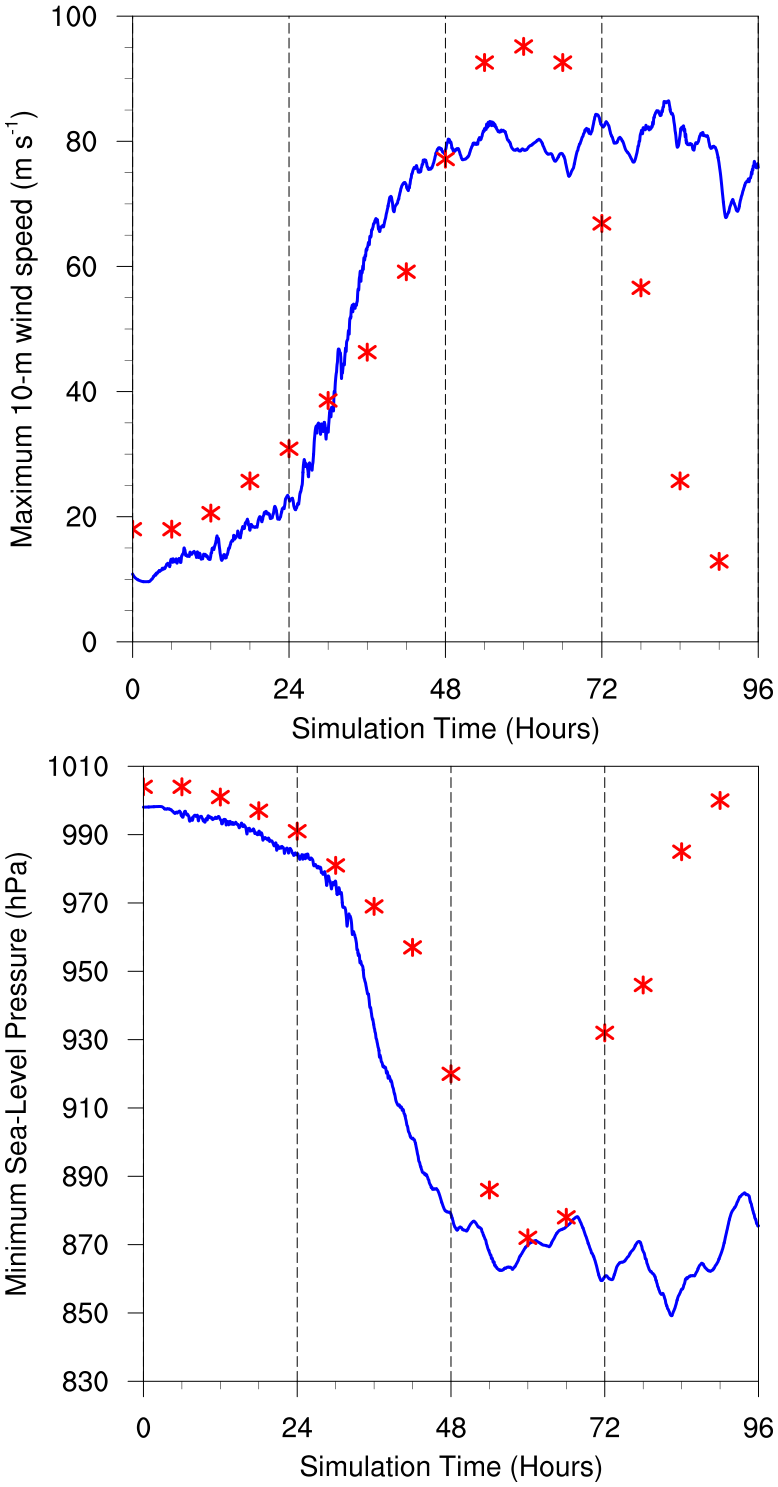
\includegraphics[width=19pc]{figures/vmax+pmin.png}}
\caption{The maximum 10-m wind speed (top panel; m s\textsuperscript{-1}) and minimum sea-level pressure (bottom panel; hPa) in the simulated storm (blue lines; plotted every minute) and from Hurricane Patricia's best track (red stars; plotted every six hours beginning at the time Patricia attained tropical storm intensity). The rapid weakening during the later stage of Patricia's lifetime was induced by landfall.}
\label{fig:vmax+pmin}
\end{figure}

%FIGURE 2%
\begin{figure}[ht]
\centerline{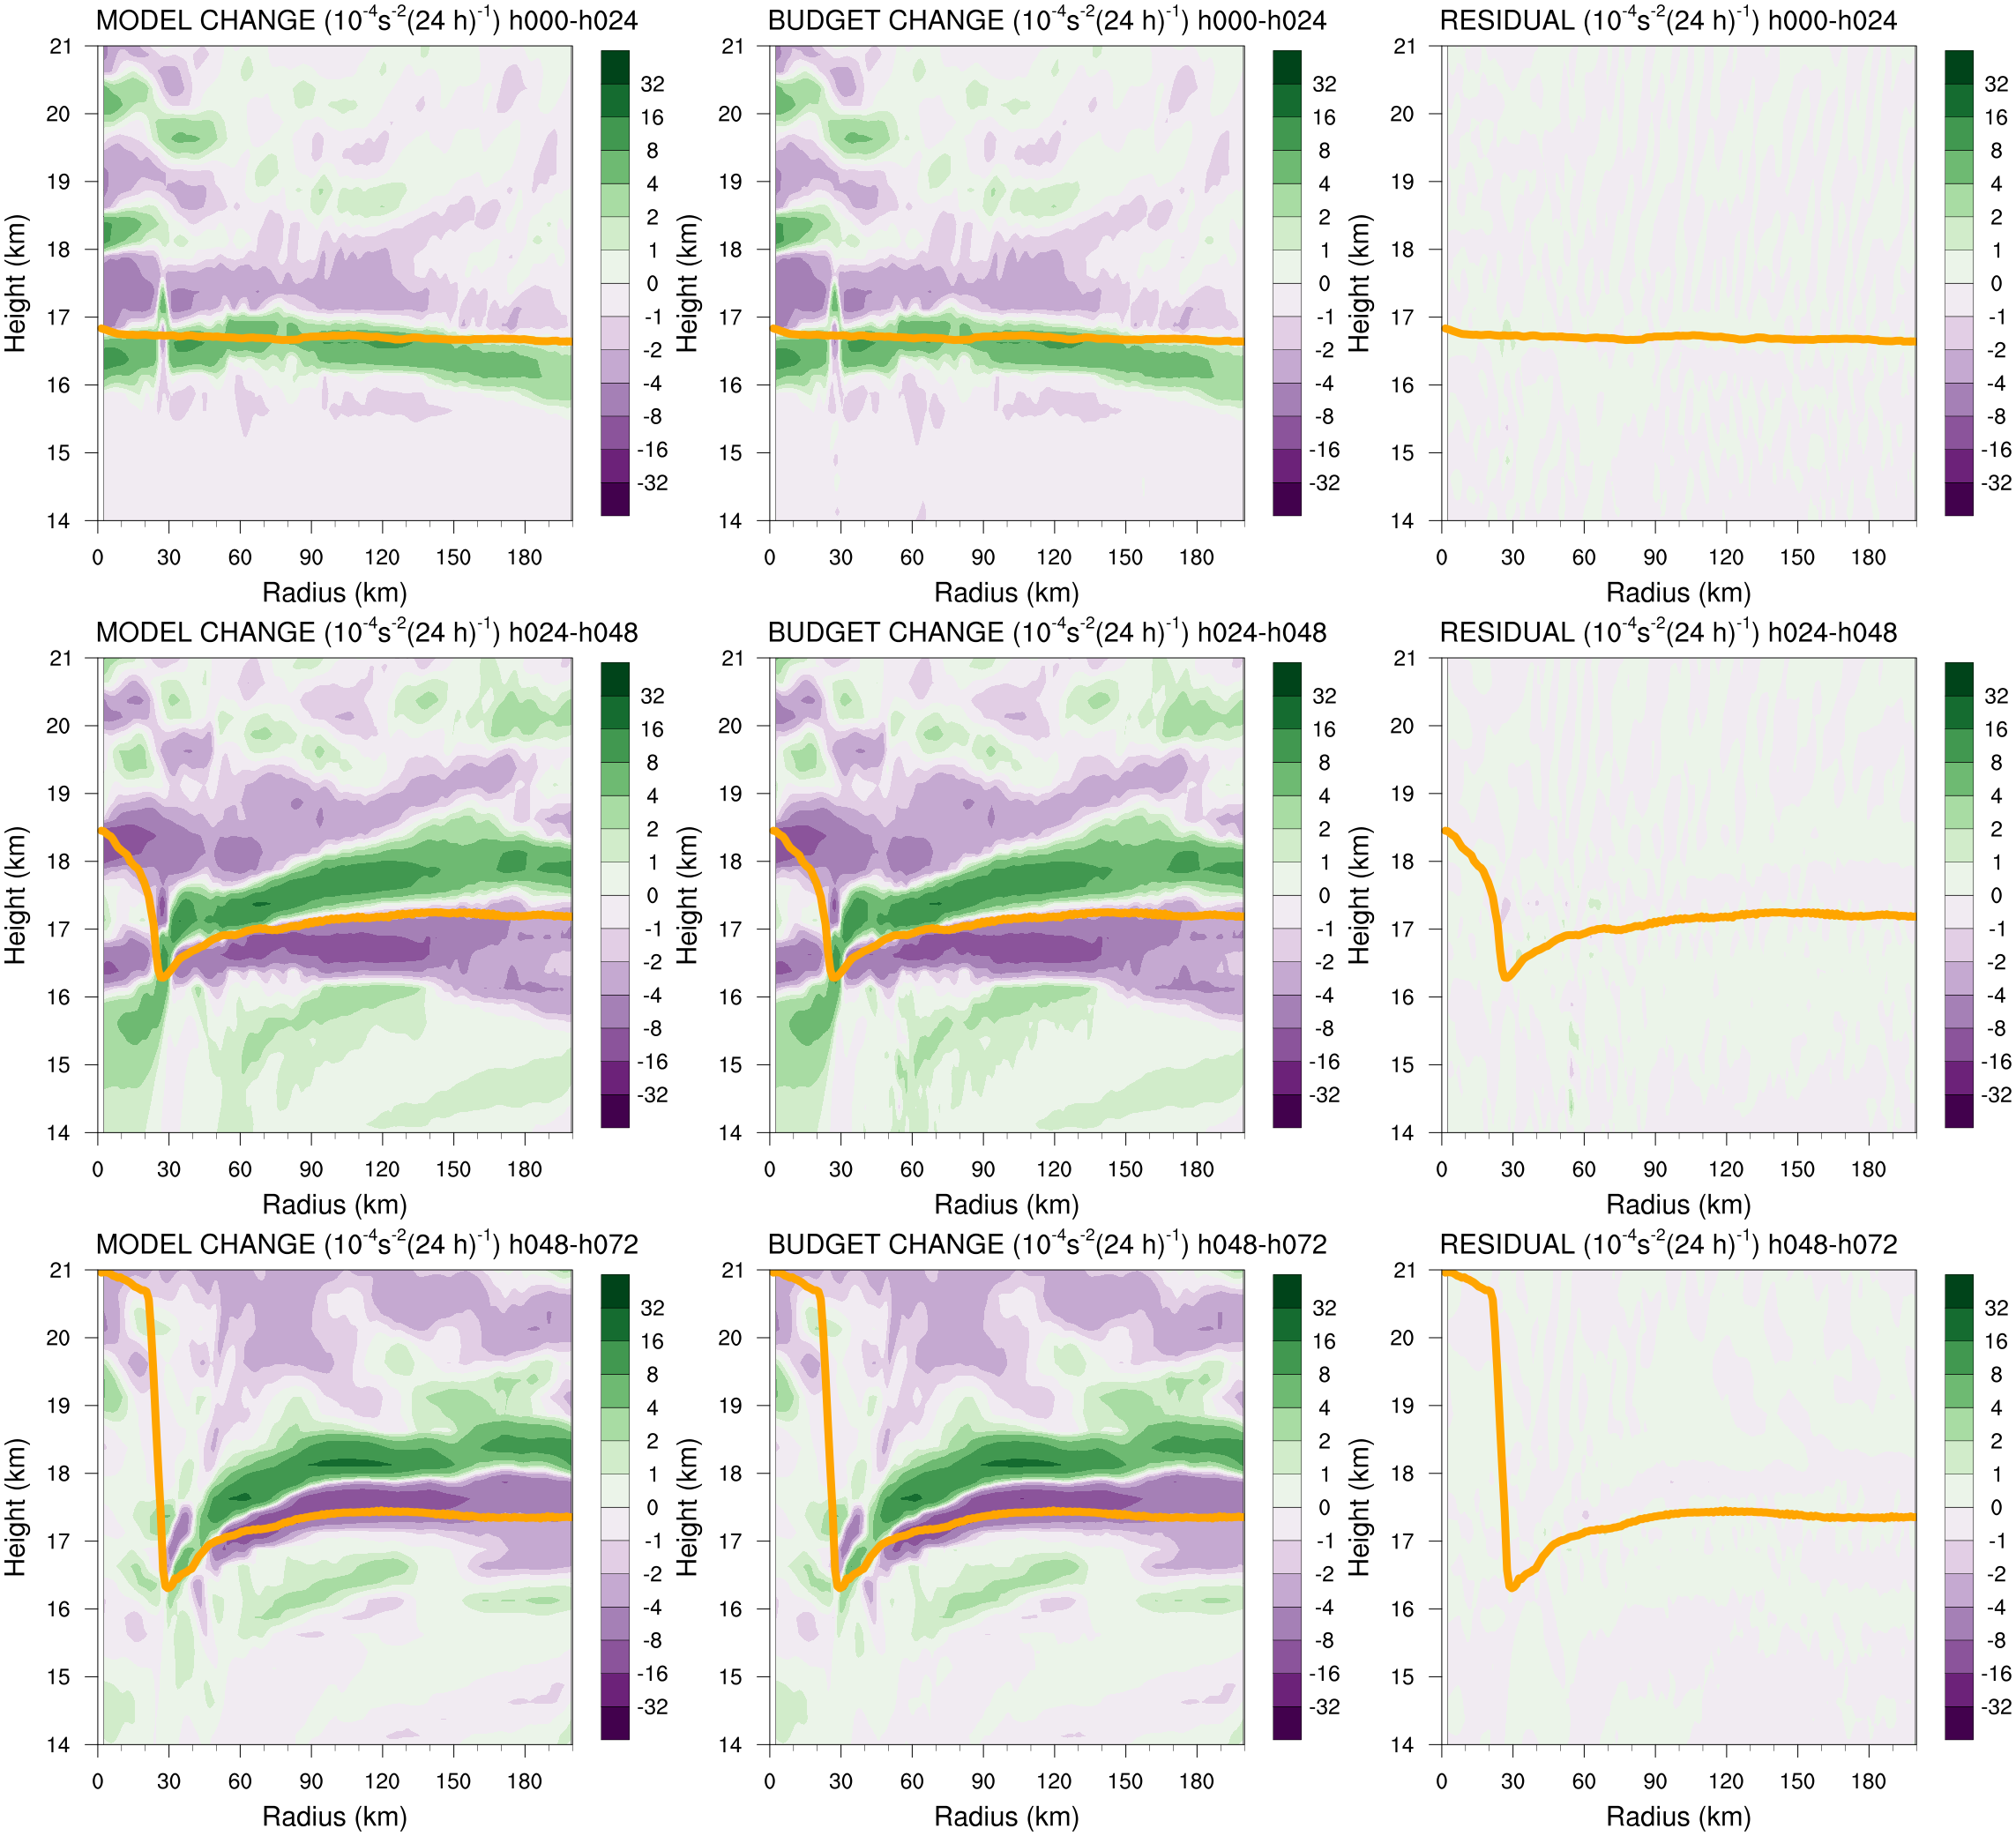
\includegraphics[width=39pc]{figures/mod+bud+res.png}}
\caption{Left panels: Twenty-four-hour changes in squared Brunt-V{\"a}is{\"a}l{\"a} frequency ($N^2$; 10\textsuperscript{-4} s\textsuperscript{-2}) computed using Eq.~\ref{eq:modelchange} over (top row) 0-24 hours, (middle row) 24-48 hours, (bottom row) 48-72 hours.
Middle Panels: The $N^2$ change over the same time periods computed using Eqs. \ref{eq:dn2dt}-\ref{eq:budgetchange}, %together with Eqs. \ref{eq:dn2dt}, \ref{eq:dthetadt}.
Right Panels: The budget residual over the same time periods, computed by subtracting the budget change (middle column) from the model change (left column).
Orange lines represent the cold-point tropopause height averaged over the same time periods.}
\label{fig:mod+bud+res}
\end{figure}

%FIGURE 3%
\begin{figure}[ht]
\centerline{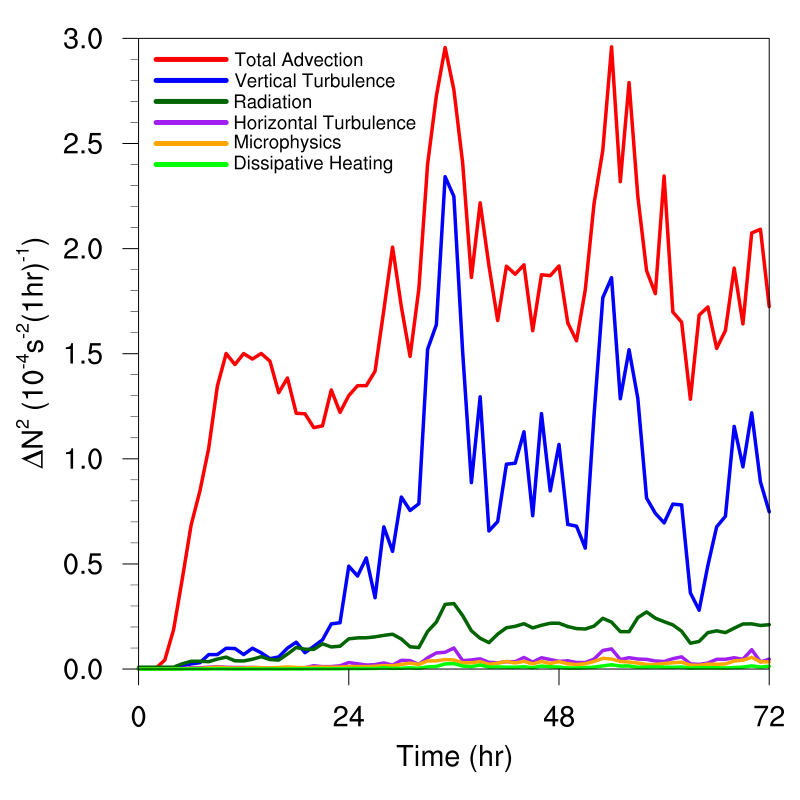
\includegraphics[width=19pc]{figures/AVG_budterms.png}}
\caption{Time series of the contribution of each of the budget terms to the time tendency of the squared Brunt-V{\"a}is{\"a}l{\"a} frequency ($N^2$; 10\textsuperscript{-4} s\textsuperscript{-2}).
For each budget term, the absolute value of the $N^2$ tendency is averaged temporally over 1-hour periods (using output every minute), and spatially in a region extending from 0 to 200 km radius and 14 to 21 km altitude.}
\label{fig:avgbudterms}
\end{figure}

%FIGURE 4%
\begin{figure*}[ht]
\centerline{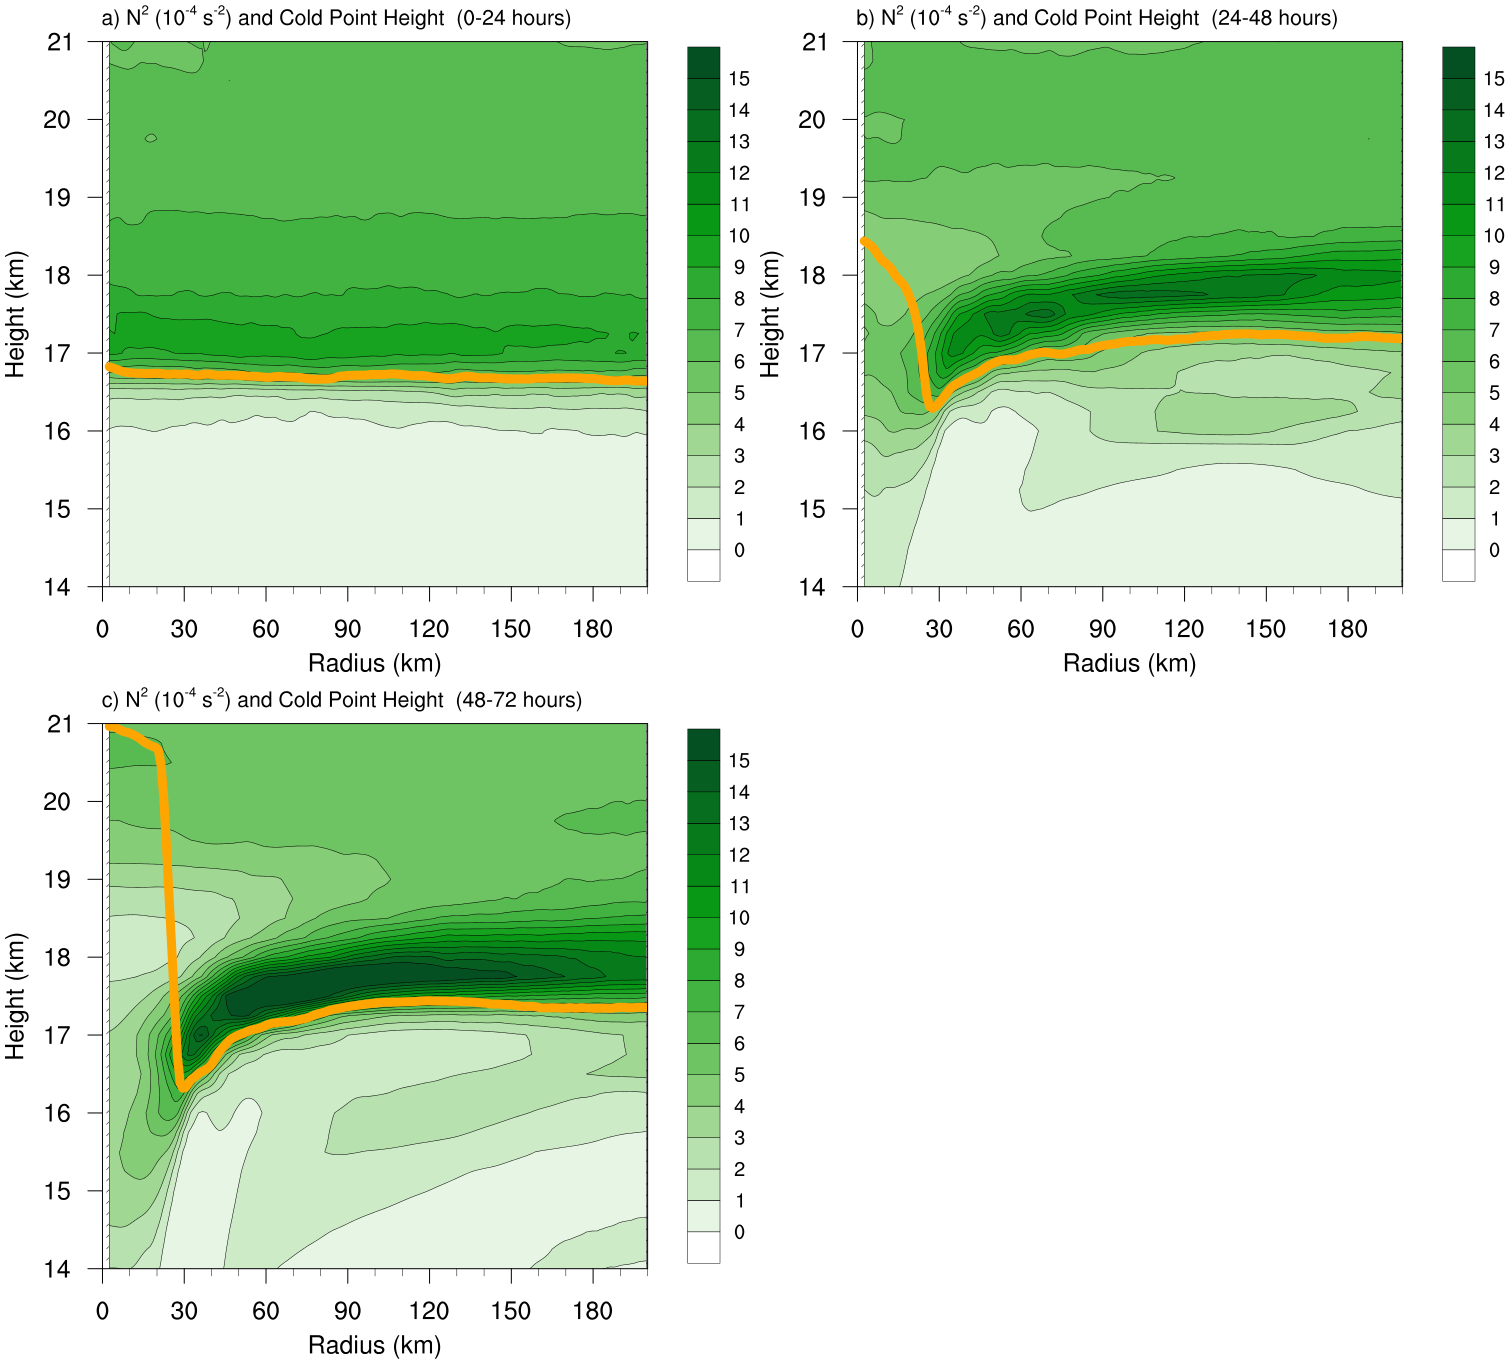
\includegraphics[width=39pc]{figures/n2-24hr-avgs.png}}
\caption{Twenty-four-hour averages of squared Brunt-V{\"a}is{\"a}l{\"a} frequency ($N^2$; 10\textsuperscript{-4} s\textsuperscript{-2}) over (a) 0-24 hours, (b) 24-48 hours, (c) 48-72 hours.
Orange lines represent the cold-point tropopause height averaged over the same time periods.}
\label{fig:n2-24hr-avgs}
\end{figure*}

%FIGURE 5%
\begin{figure*}[ht]
\centerline{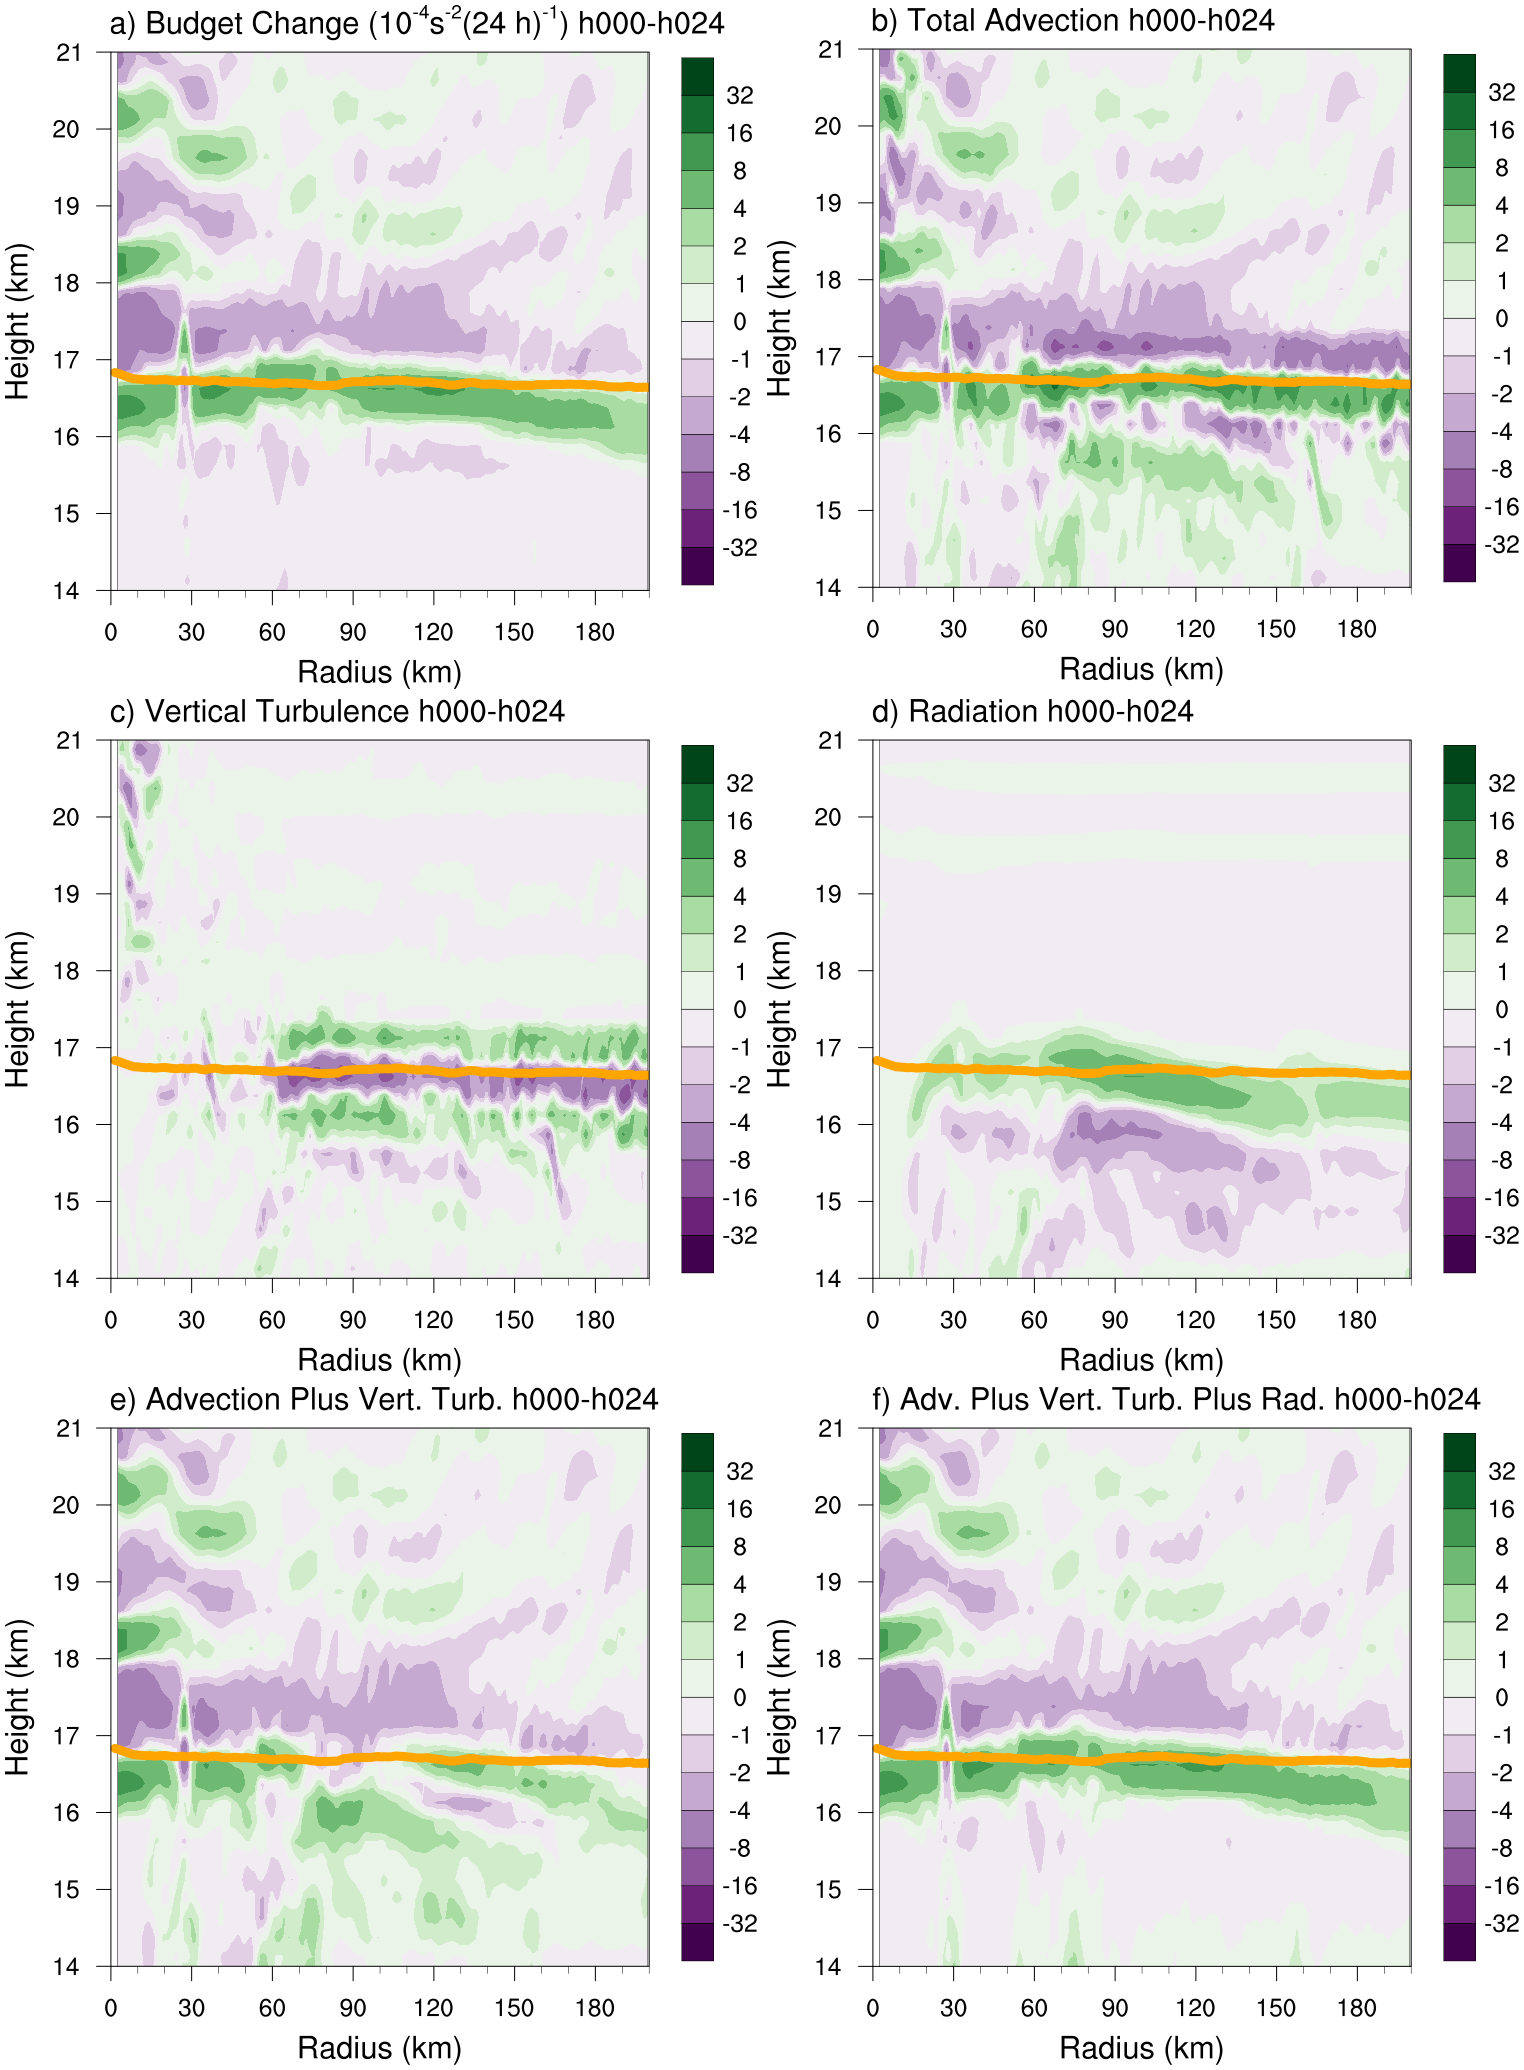
\includegraphics[width=39pc]{figures/h000-h024-budgetterms.png}}
\end{figure*}
\begin{figure}
\caption{(a) Total change in $N^2$ over the 0-24-hour period (10\textsuperscript{-4} s\textsuperscript{-2} (24 h)\textsuperscript{-1}) and the contributions to that change from (b) the sum of horizontal and vertical advection, (c) vertical turbulence, (d) longwave and shortwave radiation, (e) the sum of horizontal advection, vertical advection, and vertical turbulence, and (f) the sum of horizontal advection, vertical advection, vertical turbulence, and longwave and shortwave radiation.
Green shading indicates regions of stabilization and purple shading indicates regions of destabilization.
Orange lines represent the cold-point tropopause height averaged over the 0-24-hour period.}
\label{fig:stab-00-24}
\end{figure}

%FIGURE 6%
\begin{figure*}[ht]
\centerline{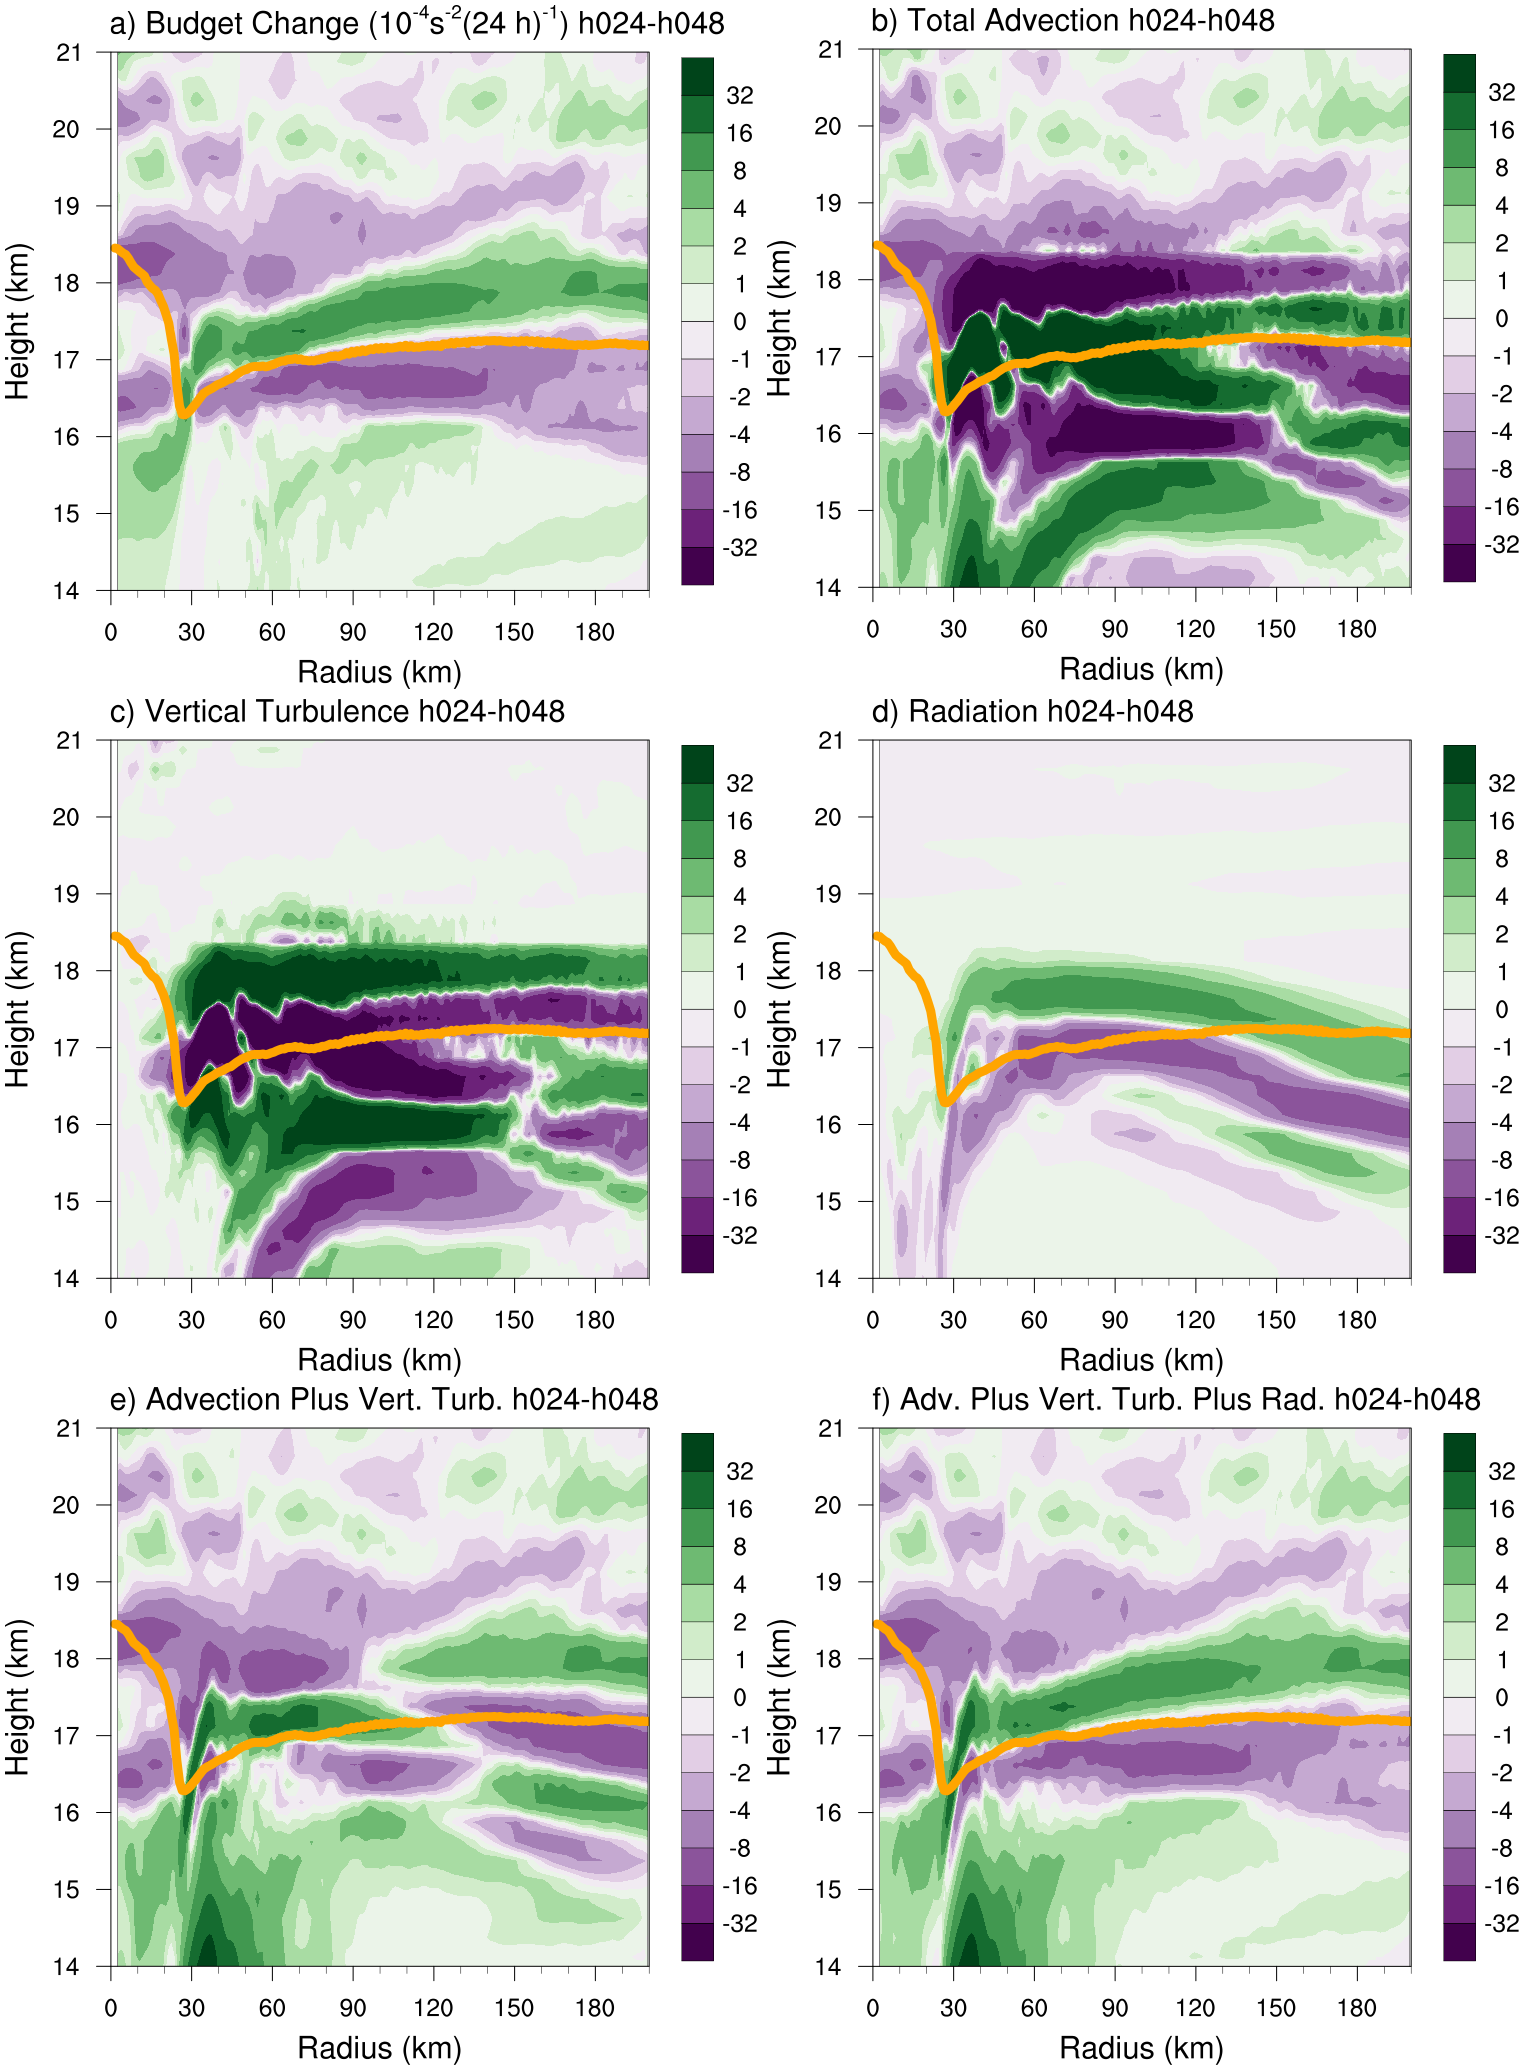
\includegraphics[width=39pc]{figures/h024-h048-budgetterms.png}}
\caption{As in Fig.~\ref{fig:stab-00-24}, but for the 24-48-hour period.}
\label{fig:stab-24-48}
\end{figure*}

%FIGURE 7%
\begin{figure*}[ht]
\centerline{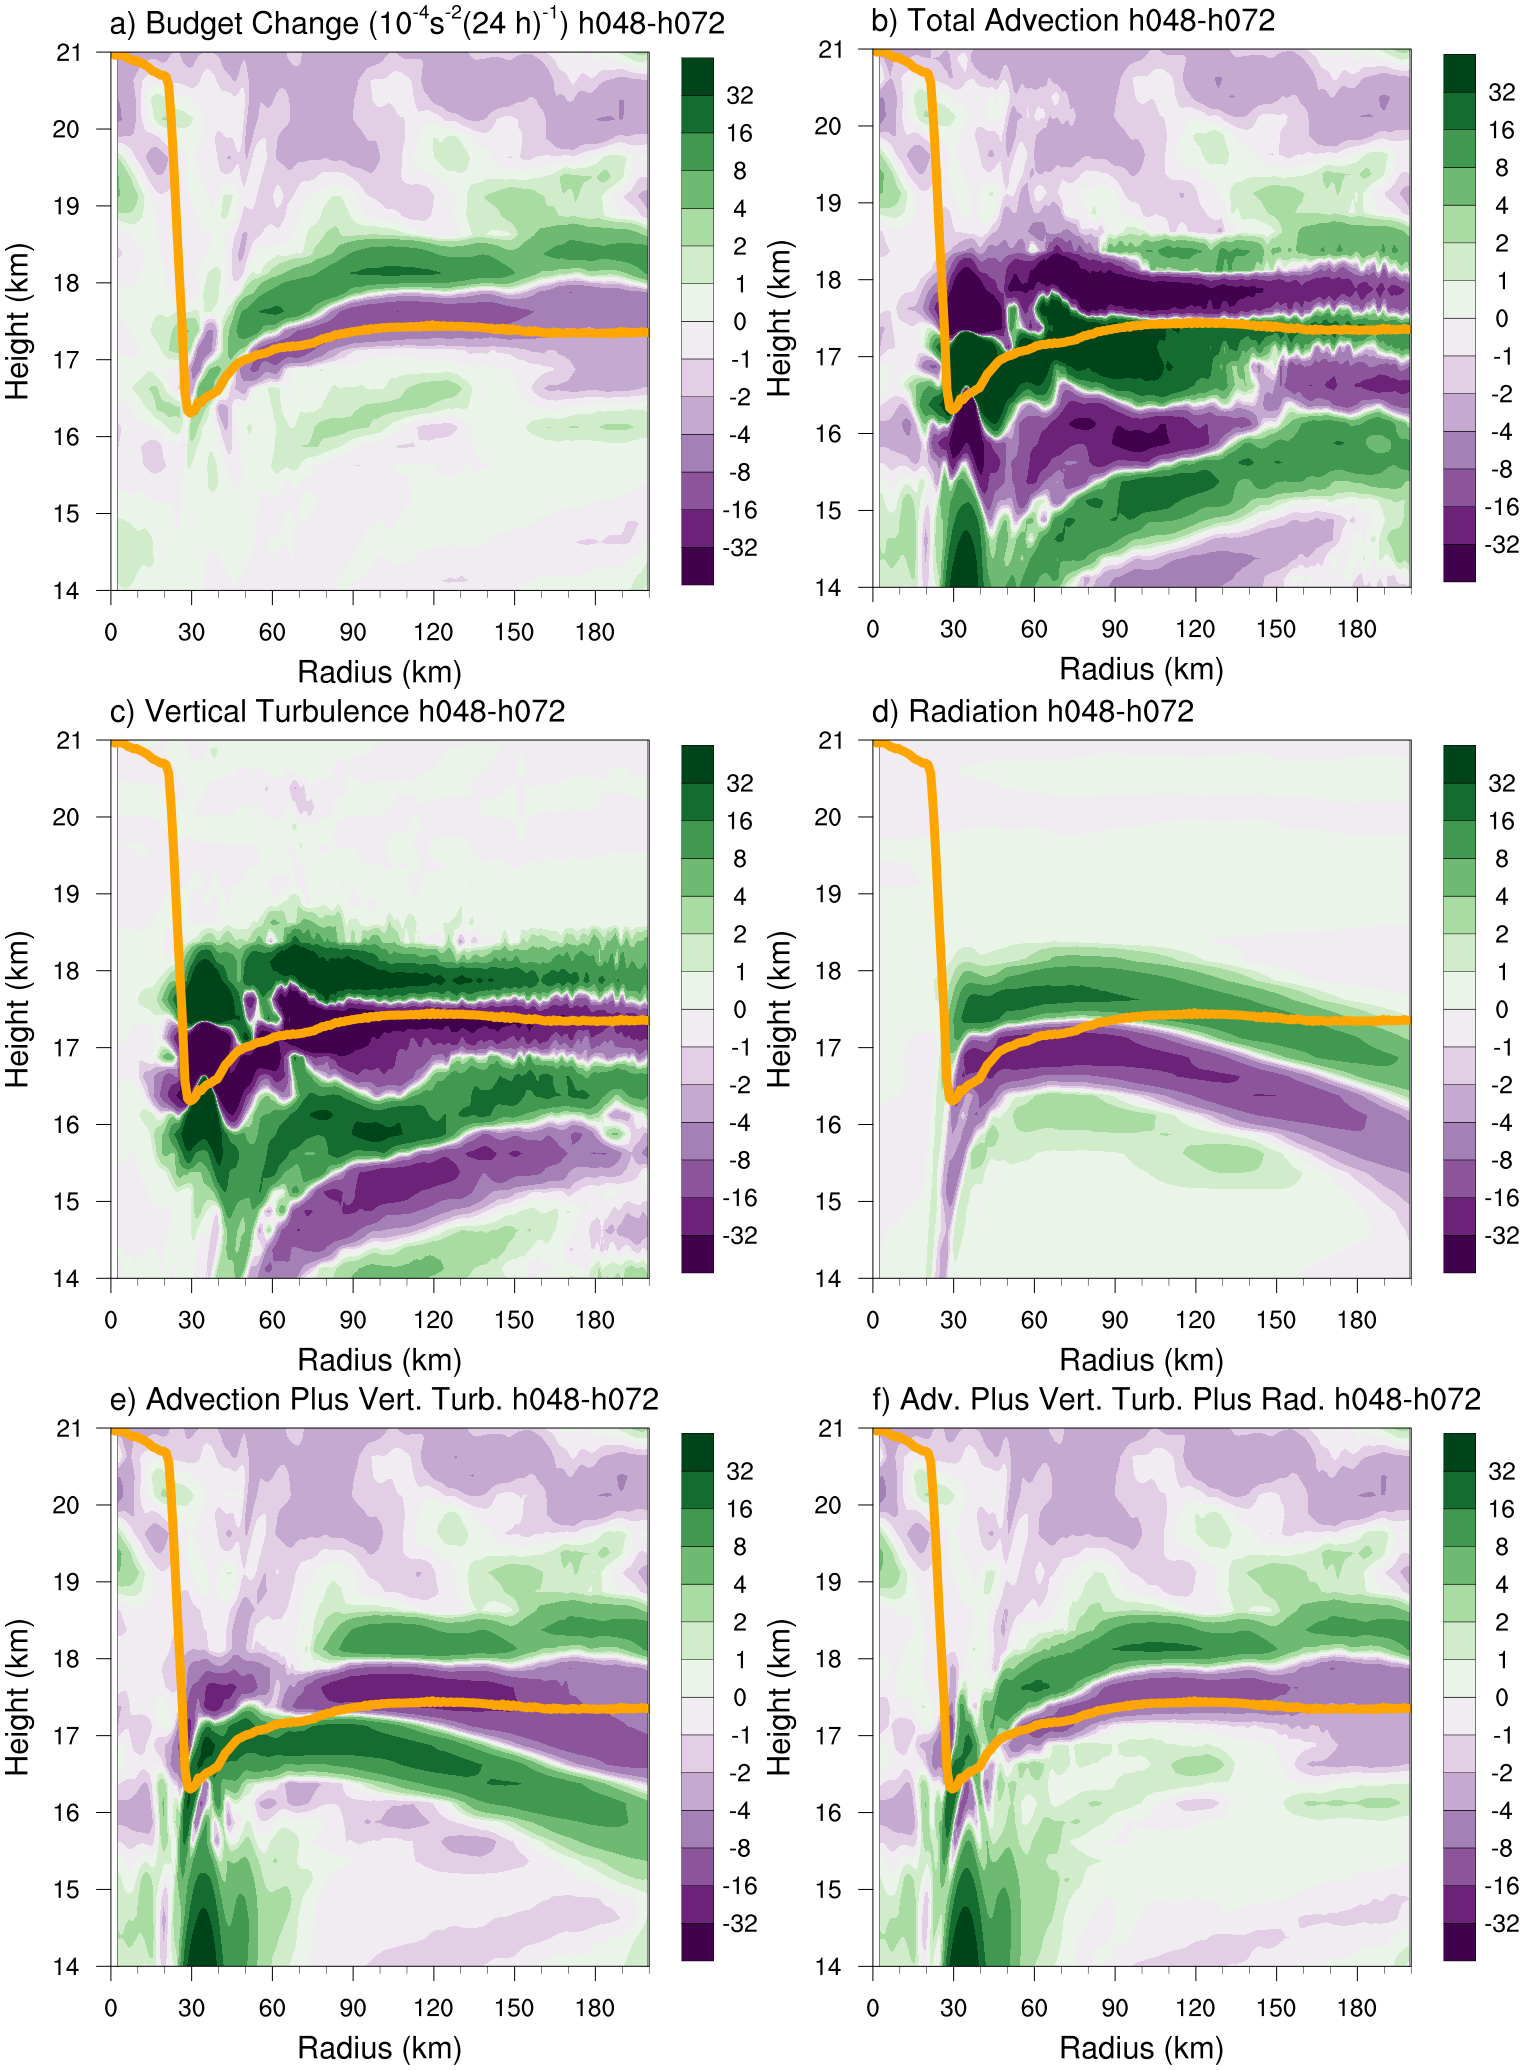
\includegraphics[width=39pc]{figures/h048-h072-budgetterms.png}}
\caption{As in Fig.~\ref{fig:stab-00-24}, but for the 48-72-hour period.}
\label{fig:stab-48-72}
\end{figure*}
